\documentclass[a4paper]{article}

%% Language and font encodings
\usepackage[english]{babel}
\usepackage[utf8x]{inputenc}
\usepackage[T1]{fontenc}

%% Sets page size and margins
\usepackage[a4paper,top=3cm,bottom=2cm,left=3cm,right=3cm,marginparwidth=1.75cm]{geometry}
\setlength{\parskip}{1em}

%% Useful packages
\usepackage{amsmath}
\usepackage{graphicx}
\usepackage[colorinlistoftodos]{todonotes}
\usepackage[colorlinks=true, linkcolor=black, urlcolor=blue]{hyperref}
\usepackage{float}
\usepackage{titlesec}
\usepackage{listings}
\usepackage{courier}
\usepackage{todonotes}
\usepackage{booktabs}
\usepackage{colortbl}

\titleformat{\paragraph}
{\normalfont\normalsize\bfseries}{\theparagraph}{1em}{}
\titlespacing*{\paragraph}
{0pt}{3.25ex plus 1ex minus .2ex}{1.5ex plus .2ex}

\begin{document}

\title{Reading time in analog clocks and watches}

\begin{titlepage}
  \centering
  \begin{figure}
    \centering
    
\includegraphics[width=0.5\textwidth]{FEUP_Logo.png}
  \end{figure}
  \vspace{1.5cm}
  {\huge\bfseries Tempo em relógios analógicos\par}
  \vspace{2cm}    
  Mário Esteves da Silva Esteves (up201607940)\par
  Ricardo Manuel Correia Magalhães (up201502862)\par
  G09
  \vfill
  {\Large Mestrado Integrado em Engenharia Informática e Computação\par}
  \vspace{1cm}
  {\large Visão por Computador\par}
  \vfill
  6 de Novembro de 2017
\end{titlepage}

\renewcommand{\contentsname}{Índice}
\tableofcontents
\newpage

\section{Introdução}

Este relatório foi realizado no âmbito da unidade curricular Visão por Computador, inserida no 1º semestre do 5º ano do Mestrado Integrado em Engenharia Informática e de Computação da Faculdade de Engenharia da Universidade do Porto. O principal objetivo deste relatório é explicar a abordagem e algoritmos escolhidos para a leitura do tempo em relógios analógicos, utilizando OpenCV e C++ para a deteção das formas das imagens.

\newpage
\section{Implementação}

Primeiramente, recorreu-se à utilização do algoritmo \textit{Canny Edge Detector}, responsável por revelar as arestas da imagem. Dessa forma, tudo o resto fica a preto, realçando-se o foco das arestas.

\begin{center}
    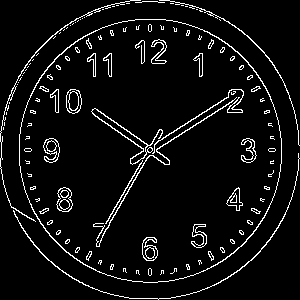
\includegraphics[scale=0.5]{canny.png}
    \\ Fig 1.: Exemplo de aplicação de Canny
\end{center}

Após a aplicação do algoritmo acima, procedeu-se à utilização de um pequeno Blur na imagem, apenas e só para se proceder à deteção da circunferência do relógio. A essa imagem desfocada foi aplicada a \textit{Circle Hough Transform}, capaz de detetar objetos circulares na imagem. De forma a diminuir o erro de se detetar círcunferências menores\footnote{Um problema comum era a deteção de círculos em algarismos mais redondos, como 3 ou 8.} na imagem, assume-se que o objeto circular com maior raio é, de facto, a borda do relógio; é calculada, também, o ponto central do relógio.

\begin{center}
    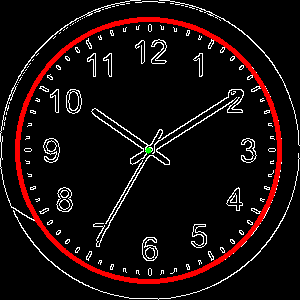
\includegraphics[scale=0.5]{outer_center.png}
    \\ Fig 2.: Exemplo de borda e centro do relógio
\end{center}

A próxima fase consiste na aplicação da \textit{Probabilistic Hough Transform}, na qual iremos obter as linhas da imagem. No entanto, todas as linhas que não estejam próximas do centro \footnote{Aplica-se um pequeno erro, dado ser difícil encontrarem-se exatamente no \textit{pixel} central.} são descartadas. Dessa forma, foram encontrada possíveis linhas para representarem os ponteiros.

\begin{center}
    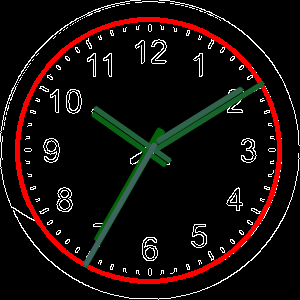
\includegraphics[scale=0.5]{detected_lines.png}
    \\ Fig 3.: Exemplo de linhas encontradas
\end{center}
\vfill
\begin{center}
    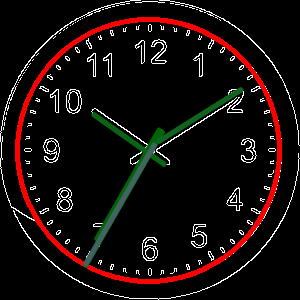
\includegraphics[scale=0.5]{possible_lines.png}
    \\ Fig 3.: Exemplo de possíveis linhas finais, perto do centro.
\end{center}

Um dos problemas encontrados foi o surgimento de linhas próximas, ambas representando o mesmo ponteiro. A nossa solução parte em percorrer as linhas próximas do centro e comparar com as outras; dessa forma, assume-se que uma linha é similar à outra caso possua o mesmo gradiente e esteja uma certa distância arbitrária. Caso uma linha possua linhas similares, é calculada a linha média da união das mesmas; caso a linha seja "independente", é automaticamente classificada como ponteiro.

Sabendo as duas ou três linhas finais, é aplicado uma ordenação do vector por ordem ascendente de comprimento da linha; ficam, por ordem, os ponteiros das horas, minutos e segundos (caso se aplique). As linhas são, então, desenhadas com cores diferentes.\footnote{Azul para as horas, verde para os minutos e vermelho para os segundos.}

Finalmente, procedeu-se ao cálculo das horas. Primeiramente, é reconhecido o ângulo de cada um dos ponteiros com recurso à função \textit{atan2}. É de notar que se aplicou uma rotação de 90º no sentido anti-horário, devido ao facto de, originalmente, os ângulos fossem referentes ao ponto 3 do relógio; assim, o ponto 12 passa a ser a referência. 

Por último, divide-se o ângulo do ponteiro das horas por 30, de forma a obter em qual dos 12 ponteiros está; por outro lado, os outros dois ponteiros são divididos por 6, de forma a conhecer-se os minutos ou segundos de 0 a 60.

\pagebreak
\section{Estado Final}

O programa final deteta, com sucesso, as horas em diversas imagens de relógio; não foi, no entanto, contemplado o uso de câmara. Foi assumido que um relógio pode ou não ter ponteiro dos segundos, sendo que o programa faz a distinção. Pode receber alguns bugs em imagens muito grandes devido aos erros arbitrários auxiliares.

\begin{center}
    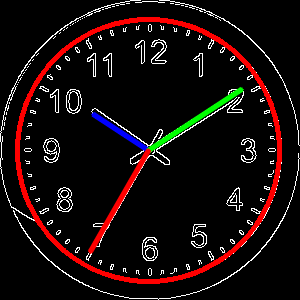
\includegraphics[scale=0.5]{final_image.png}
    \\ Fig 3.: Exemplo de imagem final.
\end{center}

\pagebreak
\section*{Anexo}
\addcontentsline{toc}{section}{Anexo}

\begin{frame}

\lstset{language=C++,
                basicstyle=\ttfamily,
                keywordstyle=\color{blue}\ttfamily,
                stringstyle=\color{red}\ttfamily,
                commentstyle=\color{green}\ttfamily,
                morecomment=[l][\color{magenta}]{\#}
}
\begin{lstlisting}
#include <opencv2/opencv.hpp>
#include <opencv2/imgproc.hpp>
#include <iostream>
#include <algorithm>
#include <math.h>

using namespace std;
using namespace cv;

int getAngle(Point p1, Point p2) {
	double angle = atan2(p1.y - p2.y, p1.x - p2.x);

	//if negative, turn it positive
	if(angle <0)
		angle+=2*CV_PI;

	angle*=180/CV_PI; //to degrees

	//change 0 degress point from right to top
	if(angle <=270)
		angle+=90;
	else
		angle-=270;

	//cout << angle << "\n";
	return angle;
}
double crossProduct(Point a, Point b) {
	return a.x*b.y - a.y*b.x;
}

double dotProduct(Point a1, Point a2, Point b1, Point b2) {
	Point vectorA(a1.x - a2.x, a1.y - a2.y), vectorB(a1.x - a2.x, a1.y - a2.y);
	return vectorA.x * vectorB.x + vectorA.y * vectorB.y;
}

double distanceBetweenPoints(Point begin,Point end) {
	return sqrt(pow(end.x-begin.x,2)+pow(end.y-begin.y,2));
}

double distanceToPoint(Point center, Point begin, Point end) {
	end -= begin;
	center -= begin;

	double area = crossProduct(center, end);
	return area / norm(end);
}

class Line {
public:
	Point begin;
	Point end;
	Point final;
public:
	Line() {}
	Line(Point begin1,Point end1, Point center) {
		begin=begin1;
		end=end1;
		if(distanceBetweenPoints(center,begin) > distanceBetweenPoints(center,end))
			final=begin1;
		else
			final=end1;
	}
};

int main( int argc, char** argv ) {
	Mat src;
	src = imread( argv[1], 1 ); //Read image file from arg

	//Check if image is loaded
	if( argc != 2 || !src.data )
	{
		printf( "No image loaded. \n" );
		return -1;
	}

	Mat dst, cdst,blur; //Additional image files

	Canny(src, dst, 50, 200, 3);
	GaussianBlur(dst, blur, Size(9, 9), 2, 2 );
	cvtColor(dst, cdst, CV_GRAY2BGR);

	//Add circles

	vector<Vec3f> circles;

	/// Apply the Hough Transform to find the circles
	HoughCircles(blur, circles, CV_HOUGH_GRADIENT, 1, blur.rows/8, 200, 100, 0, 0 );
	int max_radius=-1, circle_clock=0;

	/// Detect circle clock
	for( size_t i = 0; i < circles.size(); i++ ) {
		if(circles[i][2] > max_radius) {
			circle_clock = i;
			max_radius = circles[i][2];
		}

	}

	//Get center point + radius
	Point center(cvRound(circles[circle_clock][0]), cvRound(circles[circle_clock][1]));
	int radius = cvRound(circles[circle_clock][2]);

	//Draw outline and center
	circle( cdst, center, 3, Scalar(0,255,0), -1, 8, 0 );
	circle( cdst, center, radius, Scalar(0,0,255), 3, 8, 0 );

	vector<Vec4i> lines;
	vector<Line> potentialLines,finalLines;
	// detect the lines
	HoughLinesP(dst, lines, 1, CV_PI/180, 50, 50, 10 );
	for( size_t i = 0; i < lines.size(); i++ )	{
		Vec4i l = lines[i];
		Point begin(l[0],l[1]), end(l[2],l[3]);

		//line( cdst, begin, end, Scalar((i+5)*(i+1),100,(i+1)*(i+1)), 3, CV_AA);

		//check if is potential line by checking if it is near the center
		if(abs(distanceToPoint(center,begin,end))<3) {
			//guess which "final" point of the line is (not the center)
			//line( cdst, begin, end, Scalar((i+5)*(i+1),100,(i+1)*(i+1)), 3, CV_AA);

			potentialLines.push_back(Line(begin,end,center));
		}
	}

	cout << potentialLines.size() << "\n";

	while(!potentialLines.empty() && finalLines.size()<3){
		Line p1 = potentialLines.back();
		potentialLines.pop_back();

		vector<Line> similar;

		for(size_t i=0; i<potentialLines.size(); i++) {
			Line p2 = potentialLines[i];
			double gradient1 = (p1.final.y-center.y)/(p1.final.x-center.x);
			double gradient2 = (p2.final.y-center.y)/(p2.final.x-center.x);
			if(gradient1 == gradient2 && distanceBetweenPoints(p1.final,p2.final)<=30) {
				similar.push_back(p2);
				potentialLines.erase(potentialLines.begin()+i);
			}
		}

		if(similar.size() > 0) {
			similar.push_back(p1);
			int sumX1=0,sumX2=0,sumY1=0,sumY2=0;
			for(size_t i=0; i<similar.size(); i++) {

				sumX1+=similar[i].begin.x;
				sumX2+=similar[i].end.x;
				sumY1+=similar[i].begin.y;
				sumY2+=similar[i].end.y;
			}
			finalLines.push_back(Line(Point(sumX1/similar.size(),sumY1/similar.size()),Point(sumX2/similar.size(),sumY2/similar.size()),center));
		}
		else
			finalLines.push_back(p1);
	}
	cout << finalLines.size() << "\n";

	//sort
	Line swap;
	for (size_t c = 0 ; c < ( finalLines.size() - 1 ); c++) {
		for (size_t d = 0 ; d < finalLines.size() - c - 1; d++) {
			if (distanceBetweenPoints(finalLines[d].begin,finalLines[d].end) > distanceBetweenPoints(finalLines[d+1].begin,finalLines[d+1].end)) {

				swap       = finalLines[d];
				finalLines[d]   = finalLines[d+1];
				finalLines[d+1] = swap;
			}
		}
	}


	//Draw each pointer
	line( cdst, center, finalLines[0].final, Scalar(255,0,0), 3, CV_AA);
	line( cdst, center, finalLines[1].final, Scalar(0,255,0), 3, CV_AA);
	if(finalLines.size()==3) line( cdst, center, finalLines[2].final, Scalar(0,0,255), 3, CV_AA);

	//calculate angles
	int hourAngle = getAngle(finalLines[0].final,center);
	cout << "Hour: " << (hourAngle)/30 << "\n";

	int minutesAngle = getAngle(finalLines[1].final,center);
	cout << "Minutes: " << (minutesAngle)/6 << "\n";

	if(finalLines.size() == 3) {
		int secondsAngle = getAngle(finalLines[2].final,center);
		cout << "Seconds: " << (secondsAngle)/6 << "\n";
	}



	imshow("source", src);
	imshow("detected lines", cdst);
	waitKey();

	return 0;
}

\end{lstlisting}
\end{frame}

\end{document}